\section{Mengen}
\subsection{Definition: (Cantor)}
Unter einer Menge verstehen wir jede Zusammenfassung von bestimmten wohl unterschiedenen Objekten unserer Anschauung oder unseren Denkens zu einem Ganzen\\

\begin{figure} [H]
\centering 
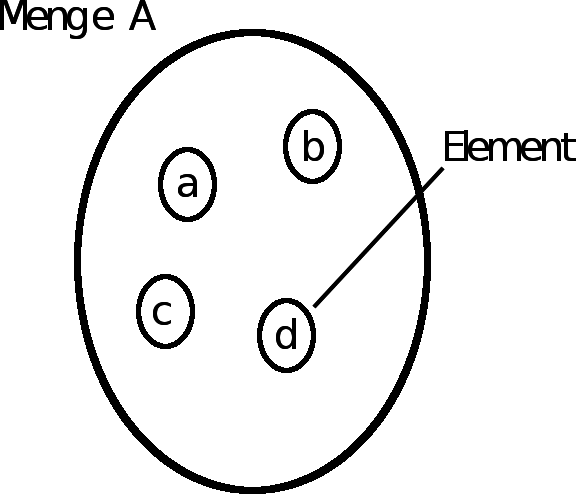
\includegraphics[width=4cm, height=3cm]{mainmatter/chapter0/pics/menge.png}
\caption{Eine einfache Menge} 
\end{figure}
\begin{equation*}
a \in A \qquad a \notin A \Leftrightarrow \neg (a \in A)
\end{equation*}
%
%
%
\subsection{Definition:}
$A, B$ Mengen 
\begin{enumerate}
\item $A \subset B \qquad \forall x \in A \Rightarrow x \in B$
\item $A \subsetneqq B \qquad (A \subset B) \wedge (A \neq B)$
\item $A = B \qquad A\subset B, \quad B\subset A$
\item $\emptyset \qquad \emptyset \subset A \quad \forall$ Mengen $A$
\item $|A| = \#A$ \qquad Anzahl der Elemente\\
 $|A| < \infty \qquad A=\{a_{1}, a_{2}, \dotsc, a_{n}\}$
\end{enumerate}
%
%
%
\subsubsection{Bemerkung:}
 \{1,2,1\} = \{1,2\}
%
%
%
\subsubsection{Beispiel:}
 \{1,2,\{1,2\},\{1,2\{1,3\}\}\}\\
gegeben Menge $M$, \quad $A=\{x \in M|x$ spricht italienisch\} = \{$x|(x \in M) \wedge x$ spricht italienisch\}\\
$\mathbb{N}=\{1,2,3, \dotsc \}$\\
$\mathbb{Z}=\{\dotsc, -1, 0, 1,2,\dotsc \} \qquad \mathbb{Z}_{\geq 0}=\mathbb{N}_{0}=\{01,2,3\cdots \}$\\
$\mathbb{Q}=\{ \frac{a}{b}|b \in \mathbb{N}, a \in \mathbb{Z}\} \frac{a}{b}=\frac{c}{d} \Leftrightarrow a \cdot d = c \cdot b$\\
$\mathbb{N}\subseteq\mathbb{Z}\subseteq\mathbb{Q}\subseteq\mathbb{R}$\\
$\mathbb{R}$ hat die Ordnung $a>b$ wenn $a$ rechts von $b$ auf dem Zahlenstrahl liegt.\\
$ a \geq b : a >b \vee a=b$\\
%
%
%
\subsection{Definition: (von weiteren Operationen auf Mengen)}

$A,B$ seien Mengen
\begin{description}
	\item[Durchschnitt: ] $A\cap B = \{x|x\in A \wedge x \in B\}$ wenn $A\cap B = 	
		\emptyset$ "` disjunkt "' $\mathop{\bigcap}\limits_{i \in I}A_{i}=\{x|x \in A$ für alle 
		$i\}$
	\item [Vereinigung: ]$A\cup B = \{x|x\in A \vee x \in B\} \mathop{\bigcup}\limits_{i \in I}A_{i}=\{x|x \in A$ für mindestens ein $i\}$
	\item[Komplement von $B$ in $A$:] $A\diagdown B = \{x|x \in A \wedge x \notin 
		B\}$
	\item[symmetrische Differenz: ] $A \bigtriangleup B = \{A \diagdown B \cup B 
		\diagdown  A\} = \{x|x\in A \cup B \wedge x \notin A\cap B\}$
	\item[Potenzmenge $P(A) = \{ B|B\subset A\}$: ] Beispiel: $A = \{1,2,3\} \quad P(A) = 
		\{\emptyset , \{1\},\{2\},\{3\},\{1,2\},\{2,3\},\{1,3\},\{1,2,3\}\}$
	\item[kartesisches Produkt: ] $ A\times B = \{(a,b)|a\in A, b\in B\}$\\
		Beispiel: $A=\{a_{1},a_{2}\}, B=\{b_{1}, b_{2}\}$\\
		$A \times B = \{(a_{1},b_{1}),(a_{1},b_{2}),(a_{2},b_{1}),(a_{2},b_{2})\}$
\end{description}

\begin{figure} [H]
\centering 
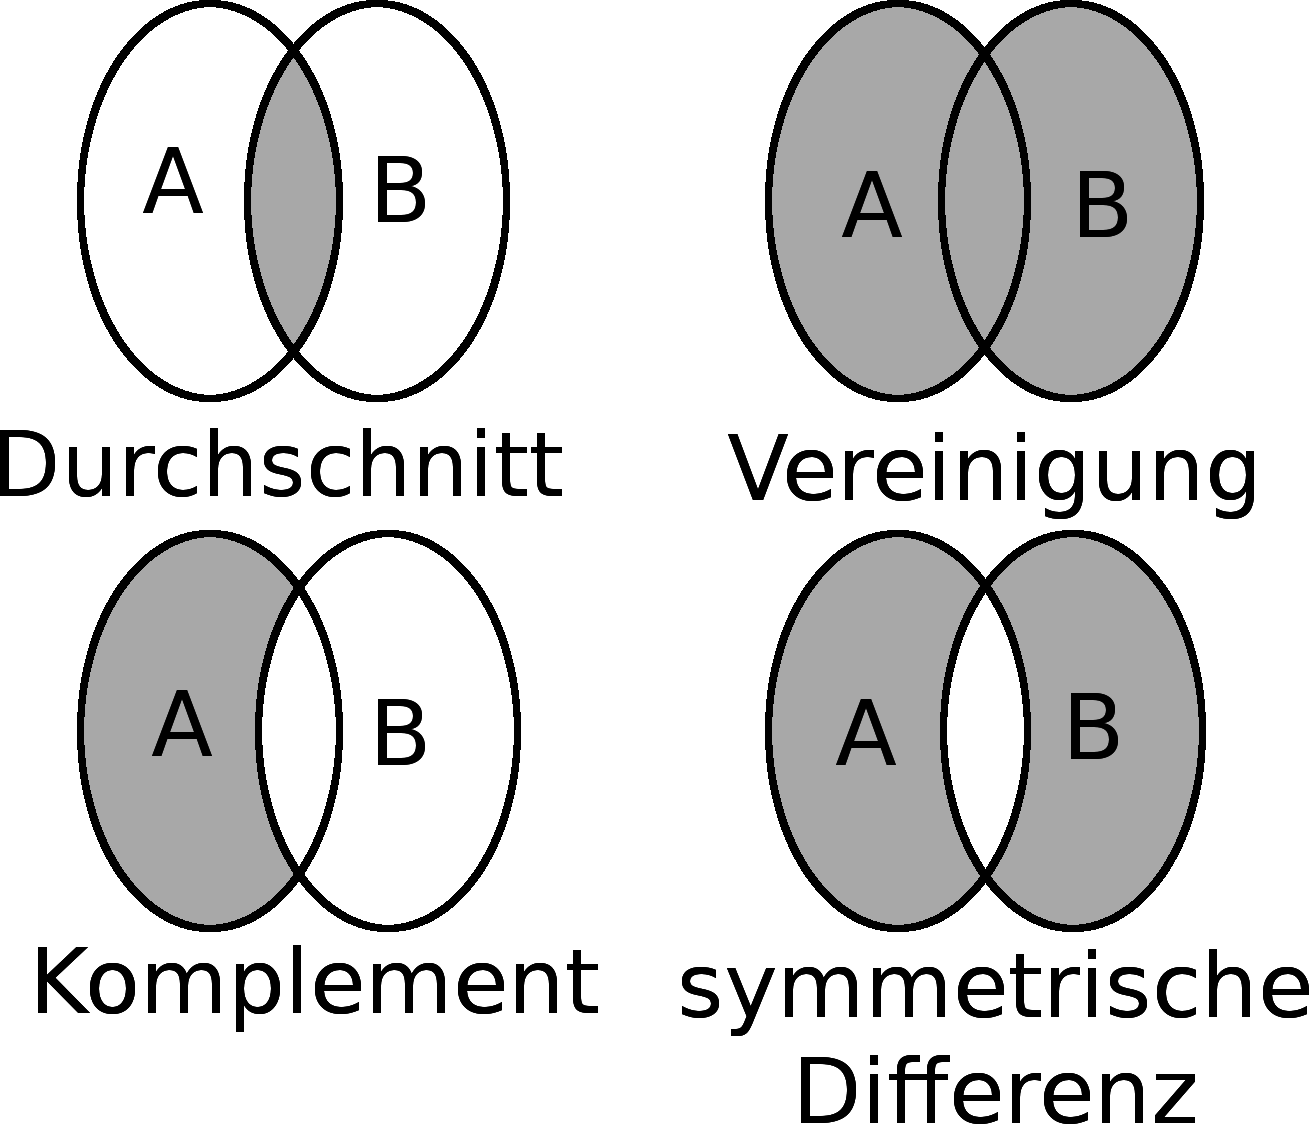
\includegraphics[width=6cm, height=6cm]{mainmatter/chapter0/pics/durchschnitt.png}
\caption{Darstellung von Operationen auf Mengen} 
\end{figure}
%
%
%
\subsection{Definition: (Relation)}
Eine Relation zwischen zwei Mengen $A$ und $B$ ist eine Teilmenge $R \subset A \times B$. Wenn $A=B$ "`Relation auf Menge A"'\\
\subsubsection{Beispiel:}
$A:$ Personen \qquad $B:$ Städte\qquad $R:$ bereits bereist\\
\begin{enumerate}[label=\alph*)]
	\item (Martin, London), (Susi, Madrid) $\in A\times B$
	\item $A=\{1,2,3,4\}$
\end{enumerate}
\begin{enumerate}
	\item $R \subset A \times A \quad R=\{(1,3),(2,1)\}$
	\item $S \subset A \times A \quad S=\{(1,1),(2,2),(3,3),(4,4)\}$ (Gleichheitsrelation)
	\item $R \subset \mathbb{R}\times\mathbb{R} \quad R=\{(a,b)|a<b\}$ 
		(Ordnungsrelation)
	\item $B=\{3,4,5,6\} \quad R=\{(3,3),(4,4)\} \subseteq A\times B$
	\item Teilerrelation auf $\mathbb{N} \quad R=\{(a,b)|a,b\in\mathbb{N}$ und $a|b\} $ 
		wobei $(a|b \mathop{\Leftrightarrow}^{\text{definiert}} b=n\cdot a, n \in 
		\mathbb{N})$
\end{enumerate}
%
%
%
\subsection{Definition: (Funktion,  $\sim$Abbildung)}
$f: A \rightarrow B$ heißt Funktion, wenn $R\subset A\times B$ Relation, bei der jedem Element aus $A$ genau einem Element aus $B$ entspricht, sodass $(a,b)\in R$.\\
Schreibweise $f(a)=b \quad f:a\mapsto b$\\
%
\begin{figure} [H]
	\centering 
	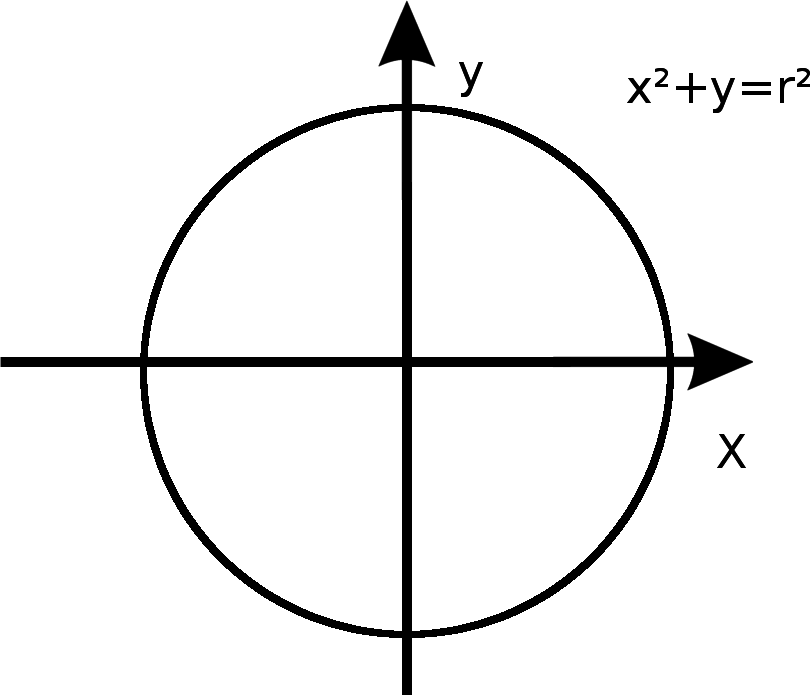
\includegraphics[width=5cm, height=4cm]{mainmatter/chapter0/pics/graphenkreis.png}
	\caption{Graphenkreis} 
\end{figure}
Jeder Graph ist eine Relation, aber nicht unbedingt eine Funktion.\\
\qquad\\
\qquad\\
%
$f: A\rightarrow B$ Funktion:
\begin{description}
	\item [] $A$ heißt Definitionsbereich von $f$
	\item [] $B$ heißt Wertebereich von $f$
	\item [] $a \in A$ heißt Argument von $f$
	\item [] $X \subset A ~ f(X)=\{b \in B|\exists a \in X$ mit $f(a)=b\}$ heißt Bildmenge 
		von	$X$ unter $f$
	\item [] $Y\subset B ~ f^{-1}(Y)=\{a \in A| f(a) \in Y\}$ heißt Urbild von $Y$
\end{description}
\subsubsection{Beispiel: }
$f: A \rightarrow A , f(a) = a$ identische Abbildung\\
$f: \mathbb{R} \rightarrow \mathbb{R}$
%
%
%
\subsection{Definition: (injektiv, surjektiv, bijektiv)}
\begin{itemize}
	\item injektiv $\forall x \neq y \in A$ gilt $f(x)\neq f(y)$
	\item surjektiv $\forall b \in B ~ \exists a \in A ~ f(a)=b$
	\item bijektiv: injektiv und surjektiv\\
		injektiv $\Leftrightarrow \forall b\in B$ gilt $|f^{-1}(b)| \leq 1$ (Jedes b hat 
		höchstens ein Urbild)\\
		surjektiv $ \Leftrightarrow \forall b \in B$ gilt $|f^{-1}(b)| \geq 1$ (Jedes b hat 
		mindestens ein Urbild)\\
		bijektiv $\Leftrightarrow \forall b \in B$ gilt $|f^{-1}(b)| = 1$ (Jedes b hat genau 
		ein Urbild)
\end{itemize}
%
\begin{figure} [H]
	\centering 
	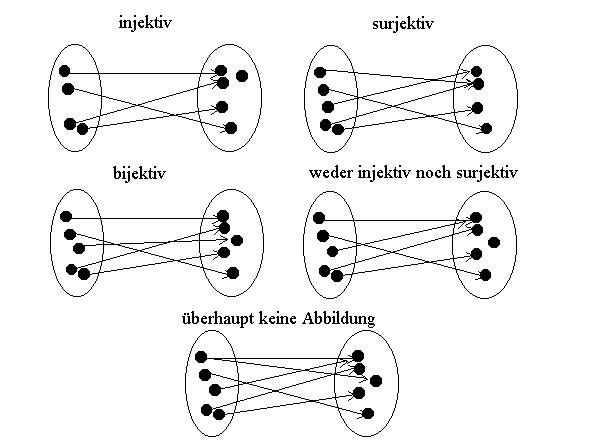
\includegraphics[width=12cm, height=6.5cm]{mainmatter/chapter0/pics/abbildungen.jpg}
	\caption{Mögliche Abbildungen auf einen Blick} 
\end{figure}